% ****** Start of file apssamp.tex ******
%
%   This file is part of the APS files in the REVTeX 4.2 distribution.
%   Version 4.2a of REVTeX, December 2014
%
%   Copyright (c) 2014 The American Physical Society.
%
%   See the REVTeX 4 README file for restrictions and more information.
%
% TeX'ing this file requires that you have AMS-LaTeX 2.0 installed
% as well as the rest of the prerequisites for REVTeX 4.2
%
% See the REVTeX 4 README file
% It also requires running BibTeX. The commands are as follows:
%
%  1)  latex apssamp.tex
%  2)  bibtex apssamp
%  3)  latex apssamp.tex
%  4)  latex apssamp.tex
%
\documentclass[%
 reprint,
%superscriptaddress,
%groupedaddress,
%unsortedaddress,
%runinaddress,
%frontmatterverbose, 
%preprint,
%preprintnumbers,
%nofootinbib,
%nobibnotes,
%bibnotes,
 amsmath,amssymb,
 aps,
%pra,
%prb,
%rmp,
%prstab,
%prstper,
%floatfix,
]{revtex4-2}
\usepackage{kotex}
\usepackage{graphicx}% Include figure files
\usepackage{dcolumn}% Align table columns on decimal point
\usepackage{bm}% bold math
\usepackage{chemformula}
\usepackage{subcaption}

%\usepackage{hyperref}% add hypertext capabilities
%\usepackage[mathlines]{lineno}% Enable numbering of text and display math
%\linenumbers\relax % Commence numbering lines

%\usepackage[showframe,%Uncomment any one of the following lines to test 
%%scale=0.7, marginratio={1:1, 2:3}, ignoreall,% default settings
%%text={7in,10in},centering,
%%margin=1.5in,
%%total={6.5in,8.75in}, top=1.2in, left=0.9in, includefoot,
%%height=10in,a5paper,hmargin={3cm,0.8in},
%]{geometry}

\begin{document}


\title{캐털레이스의 반응속도 결과보고서}

\author{서울대학교 전기정보공학부 2018-12432 박정현}
 \email{alexist@snu.ac.kr}
\date{실험일자: 10/10/2023, 제출일자 : 10/15/2023}% It is always \today, today,
             %  but any date may be explicitly specified

\begin{abstract}
본 실험에서는 식물의 세포의 퍼옥시즘에서 과산화수소의 분해의 촉매로 작용하는 효소  카탈레이즈를 활용하여 산소기체의 발생 속도를 과산화수소의 농도에 따라 측정하고 Michaelis–Menten equation와 효소 및 촉매에 대한 이해도를 높인다. 낮은 농도에서 오차가 발생하는 이유, 그리고 이를 해결하기 위한 해결법, 그리고 산소 기체 생성량을 측정하는 새로운 방법을 제시하였다.
\end{abstract}

%\keywords{Suggested keywords}%Use showkeys class option if keyword
                              %display desired
\maketitle

%\tableofcontents

\section{\label{sec:level1}Assignment}
\subsection{\label{sec:level2} 1}
아래의 화학반응에서 화학반응 속도는 다음과 같다.
\begin{align}
	\ch{A} &{\overset{k_{1}}{\longrightarrow}} \ch{B}\\
	\frac{d[\ch{B}]}{dt} &= k_{1}[\ch{A}]
\end{align}

아레니우스 식에 의해 $k_{1}$은 식(\ref{eq:arrneiuos})와 같이 나타난다. 여기서 $E_{a}$는 아레니우스 에너지이고 $A$는 $k_{1}$와 같은 차원을 가지는 상수이다. 따라서 온도가 상승함에 따라 $k_{1}$은 증가하게 되고 화학 반응속도는 증가하게 된다. 하지만 온도가 증가함에 따라 단백질은 변성이 일어나게 되면서 단백질의 구조가 바뀌므로 enzyme이 작용하기 위한 key와 lock 관계가 사라지게 되어 activity가 감소하게 된다. [3] 

\begin{align}
	k_{1} &= A\exp\left(-\frac{E_{a}}{RT}\right)\label{eq:arrneiuos}
\end{align}

Protein은 4개의 level을 가지고 있다. Primary structure은 아미노산의 배열, secondary structure은 primary structure의 아미노산들이 서로 상호작용하여 단백질이 나선형, 혹은 평면형으로 배열을 이루는 것이며 각각을 $\alpha-helix$, $\beta-strand$이라고 한다. Tertiary structure는 secondary structure사이의 상호작용으로 3차원 구조를 이룬 단백질 구조이며 Quaternary Structure은 하나 이상의 chain이 존재하는 경우의 단백질이다.[5]
\begin{figure*}[htbp]
	\begin{subfigure}{0.4\textwidth}
		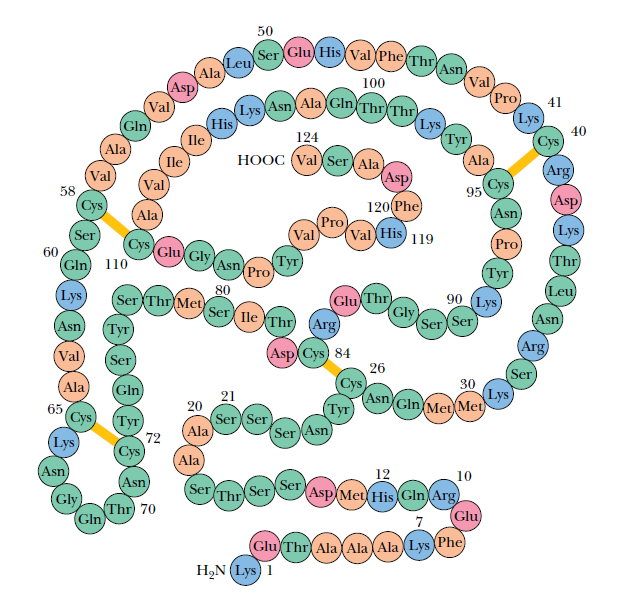
\includegraphics[width = 0.5\linewidth]{First.png}% Here is how to import EPS art
		\caption{\label{fig:First}Primary structure}
	\end{subfigure}
	\begin{subfigure}{0.4\textwidth}
		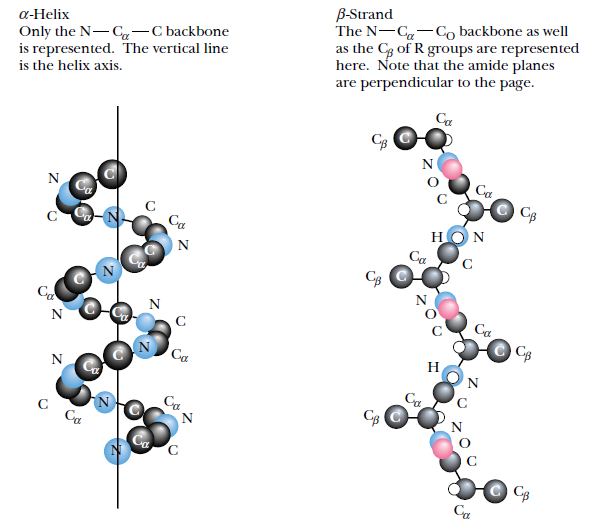
\includegraphics[width = 0.5\linewidth]{Second.png}% Here is how to import EPS art
		\caption{\label{fig:Second}Secondary structure}
	\end{subfigure}

	\begin{subfigure}{0.4\textwidth}
		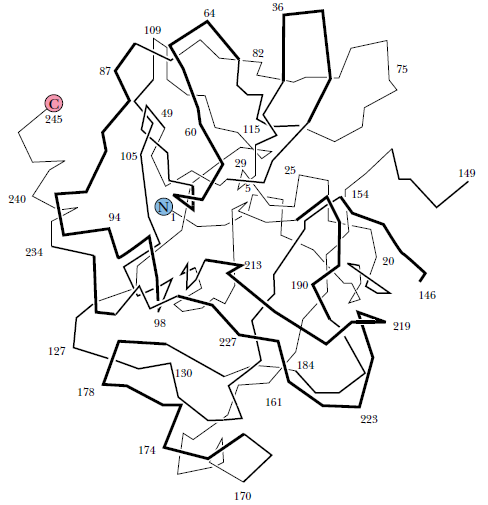
\includegraphics[width = 0.5\linewidth]{Third.png}% Here is how to import EPS art
		\caption{\label{fig:Third}Tertiary structure}
	\end{subfigure}
	\begin{subfigure}{0.4\textwidth}
		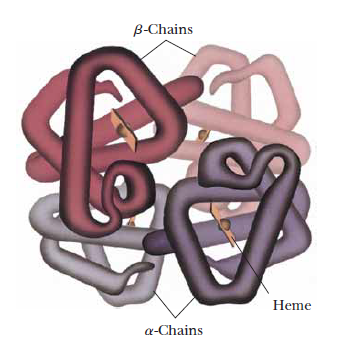
\includegraphics[width = 0.5\linewidth]{Fourth.png}% Here is how to import EPS art
		\caption{\label{fig:Fourth}Quaternary Structure}
	\end{subfigure}
	\caption{\label{fig:Protein}여러 protein구조 }
\end{figure*}

깁스에너지는 $\Delta G = \Delta H - T \Delta S$이다. 아미노산 사이의 이온 결합, 수소결합, 분산력과 같은 결합력은 $\Delta H$를 낮추게 된다. 따라서 저온에서는 작은 $\Delta S$에도 불구하고 아미노산들 사이 가장 많은 상호작용을 하는 tertiary structure,  quaternary structure와 같이 꼬여 있는 상태가 더 안정한 상태이다. 하지만 온도가 증가함에 따라 $\Delta S$에 의한 영향이 증가하게 된다. 이때 꼬여 있는 상태가 아닌 풀어져 있는 protein의 상태가 더 낮은 깁스에너지를 가지게 된다. 따라서 Fig.\ref{fig:denaturation}와 같이 단백질의 구조가 붕괴되는 denaturation가 발생하게 된다.[3][6]

\begin{figure}[htbp]
	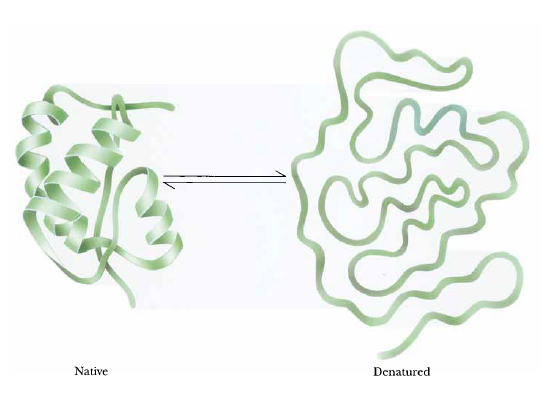
\includegraphics[width = 0.6\linewidth]{denaturation.png}% Here is how to import EPS art
	\caption{\label{fig:denaturation}Denaturation}
\end{figure}

\subsection{\label{sec:level2} 2}
효소와 함께 생성되는 물질의 생성 속도를 나타내는 식(Michaelis–Menten equation)은 식(\ref{eq:mich})와 같다.[2] 단, $[\ch{E}]$는 촉매, $[\ch{S}]$는 반응하는 기질의 농도이다.
\begin{align}
	v &= k_{2}[\ch{ES}] = \frac{k_{2}[\ch{E}]_{0}[\ch{S}]}{[\ch{S}] + K_{m}}\label{eq:mich}
\end{align}

라인웨버-버크 식(Lineweaver-Burk equation)은 식 (\ref{eq:line}) 와 같다.[1] $[\ch{S}]$가 감소함에 따라 반응속도 $v$가 감소함을 알 수 있다. 따라서 $[\ch{S}]$가 최대 값을 가질 때 속도 또한 최대이므로 $[\ch{S}] = \infty$로 두는 경우 최대 속도는 식 (\ref{eq:max})와 같다.

\begin{align}
	\frac{1}{v} &= \frac{1}{k_{2}[\ch{E}]_{0}} + \frac{K_{m}}{k_{2}[\ch{E}]_{0}[\ch{S}]}\label{eq:line}
\end{align}

\begin{align}
	v_{max} &= k_{2}[\ch{E}]_{0} \label{eq:max}\\
	&= 8\times 10^{5}\times 5 \times 10^{-5}M/s\\
	&= 40 [M/s]
\end{align}

최대 속도의 $0.2$배인 경우 식(\ref{eq:mich2})을 만족한다.
\begin{align}
	\begin{split}
		0.2v_{max} &= 0.2 k_{2}[\ch{E}]_{0}\\
		&=\frac{k_{2}[\ch{E}]_{0}[\ch{S}]}{[\ch{S}] + K_{m}}\label{eq:mich2}
	\end{split}
\end{align}

따라서 $[\ch{S}]$는 아래의 식을 만족한다.

\begin{align}
	\frac{[\ch{S}]}{[\ch{S}] + K_{m}} &= 0.2\\
	[\ch{S}] &= \frac{K_{m}}{4}\\
	&= 1\times 10^{-5} [M]
\end{align}

\section{\label{sec:level1}Data \& Result}
\subsection{\label{sec:level2} 1}
시간에 따라 생성된 산소원자의 몰값은 Fig.\ref{fig:v_t}와 같다. 단, 산소원자의 몰값은 이상기체임을 가정하고 $n=\frac{P_{\ch{O2}}V}{RT}$를 이용해 계산하였다. 이때 실험에 사용된 삼각플라스크의 부피는 $100mL$, 그리고 그외의 상수들은 $R=8.3145J/mol K$, $T=300K$으로 두고 계산하였다. 단, 실험 장비에서 측정단위가 $hPa$이므로 $Pa$로 변환하였다. 또한 산소기체가 빠져나가는 것을 고려하여 증가하는 압력중 가장 높은 기울기를 가지고 $R^{2}$이 가장 1에 가까운 데이터를 추출하여 기울기를 계산하였다.

\begin{figure*}[htbp]
	\begin{subfigure}{0.4\textwidth}
		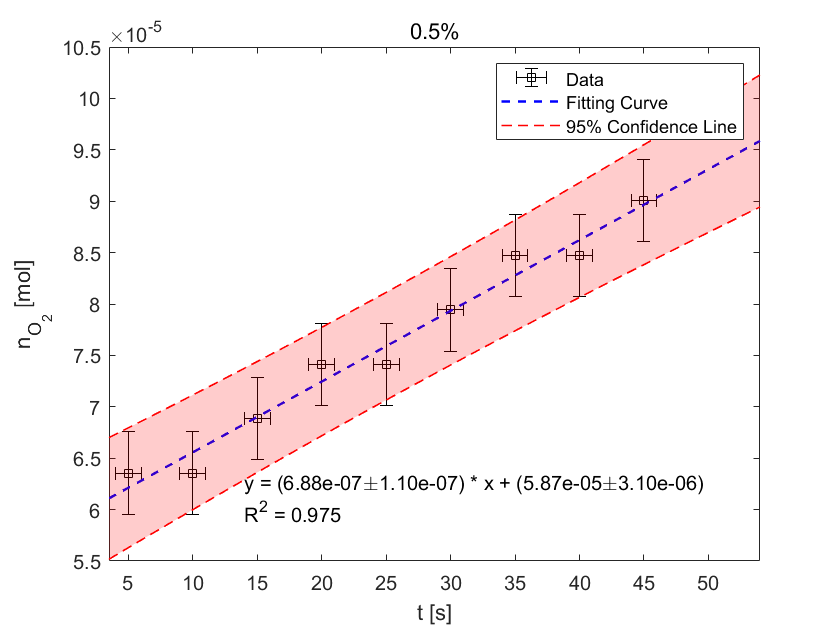
\includegraphics[width = 1\linewidth]{MOL_05.png}% Here is how to import EPS art
		\caption{\label{fig:MOL_05}0.5\% $\ch{H2O2}$}
	\end{subfigure}
	\begin{subfigure}{0.4\textwidth}
		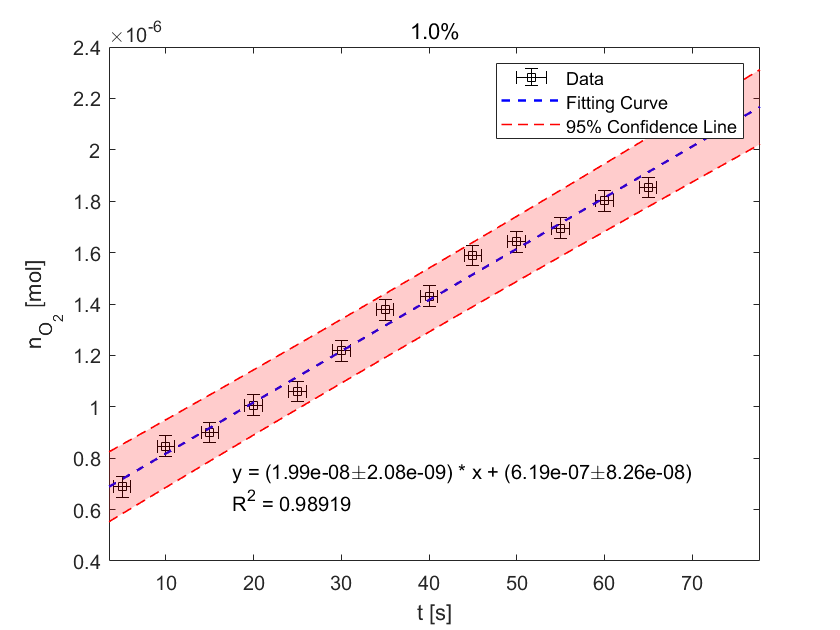
\includegraphics[width = 1\linewidth]{MOL_10.png}% Here is how to import EPS art
		\caption{\label{fig:MOL_10}1.0\% $\ch{H2O2}$}
	\end{subfigure}

	\begin{subfigure}{0.4\textwidth}
		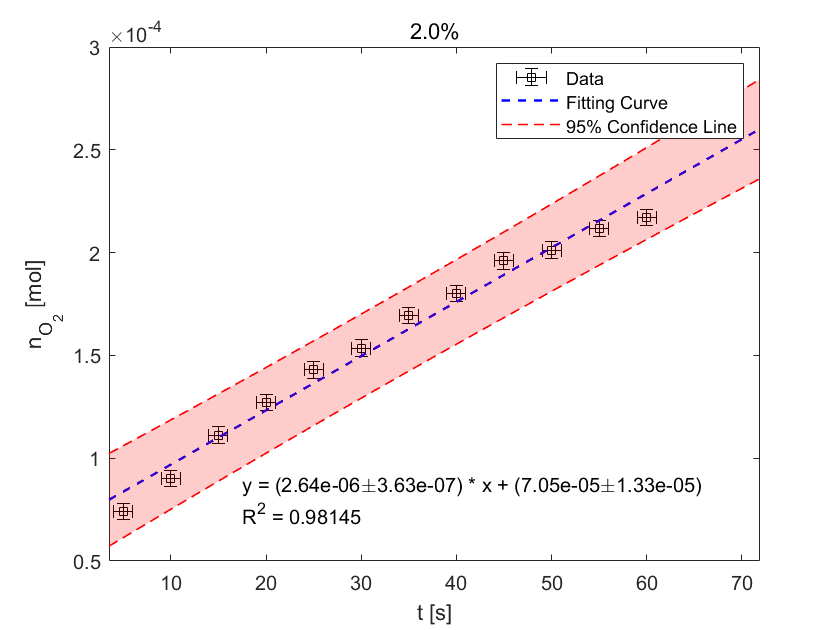
\includegraphics[width = 1\linewidth]{MOL_20.png}% Here is how to import EPS art
		\caption{\label{fig:MOL_20}2.0\% $\ch{H2O2}$}
	\end{subfigure}
	\begin{subfigure}{0.4\textwidth}
		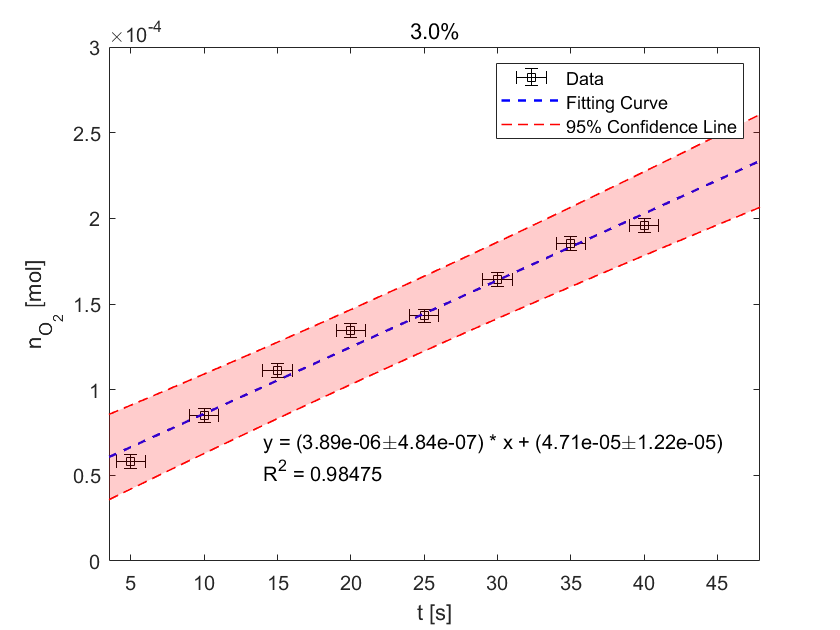
\includegraphics[width = 1\linewidth]{MOL_30.png}% Here is how to import EPS art
		\caption{\label{fig:MOL_30}3.0\% $\ch{H2O2}$}
	\end{subfigure}

	\begin{subfigure}{0.4\textwidth}
		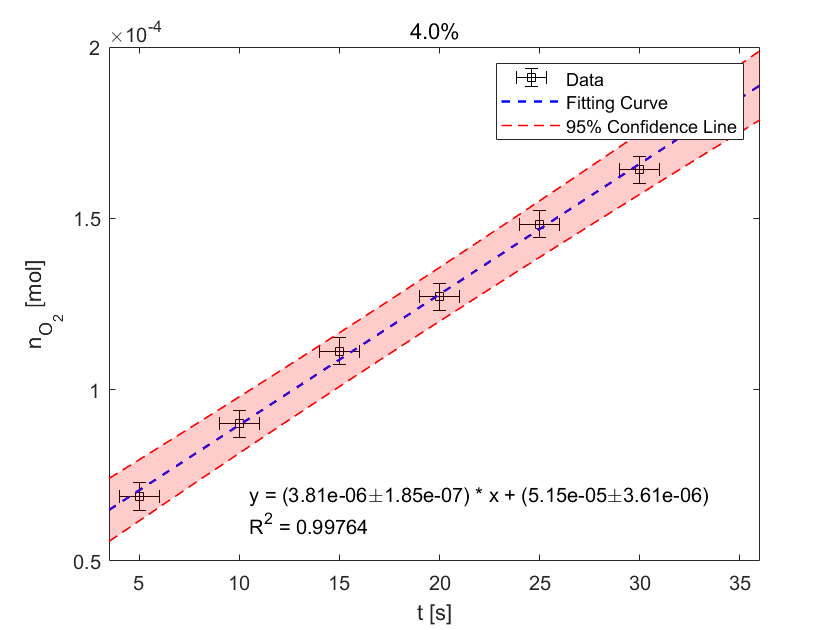
\includegraphics[width = 1\linewidth]{MOL_40.png}% Here is how to import EPS art
		\caption{\label{fig:MOL_40}4.0\% $\ch{H2O2}$}
	\end{subfigure}
	\begin{subfigure}{0.4\textwidth}
		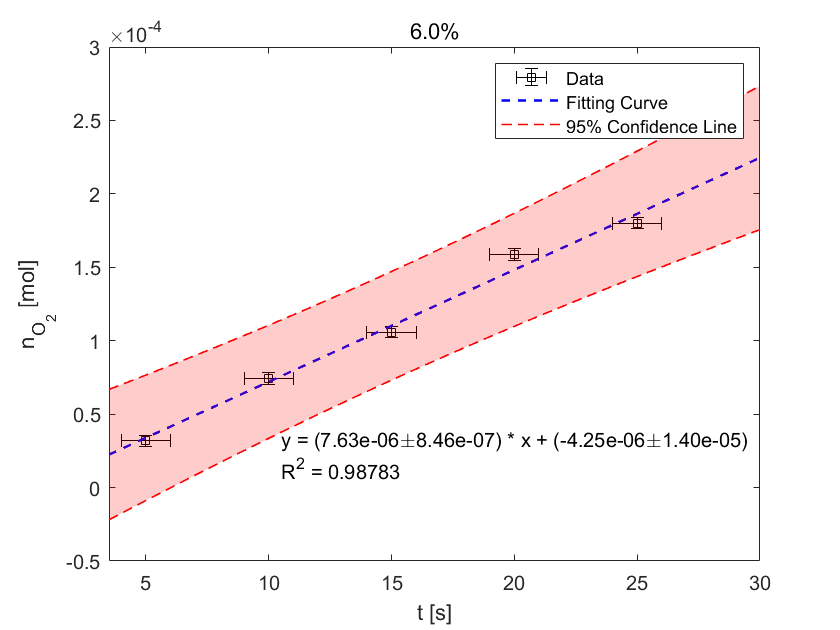
\includegraphics[width = 1\linewidth]{MOL_60.png}% Here is how to import EPS art
		\caption{\label{fig:MOL_60}6.0\% $\ch{H2O2}$}
	\end{subfigure}
	\caption{\label{fig:v_t}Generate Oxide mole value versus time}
\end{figure*}

기울기를 통해 계산된 속도를 통해 $1/v$, $1/[H_{2}O]$에 대한 그래프는 Fig.\ref{fig:TOT}와 같다. 단, 여기서 $[H_{2}O]$는 반응을 통해 생성된 물의 농도이다. 이 때 화학반응과 생성된 물의 농도는 아래의 관계식 (\ref{eq:rel})을 만족한다. 투입된 카타레이스의 부피와 $\ch{H2O2}$의 부피가 각각 $2mL$, $30mL$이므로 총부피는 $V_{liq}=0.032L$을 대입하여 계산하였다. 이 때 $0.5\%$ $\ch{H2O2}$데이터의 경우 측정 다른 농도의 측정 값으로부터 먼거리에 떨어져 있어 큰 오차를 발생시켜 해당 데이터를 포함한 경우와 포함하지 않은 경우에 대해 모두 fitting하였으며 각각에 대한 그래프는  Fig.\ref{fig:TOT_w_05}, \ref{fig:TOT_wo_05}와 같다. 각각에 대한 결과로 부터 Michaelis constant $K_{m}$을 계산하면 Tab.\ref{tab:KM}, 측정된 $V_{max}$값은 Tab.\ref{tab:VMAX}와 같다. 카탈레이스를 가열한 후 $6\%$의 $\ch{H2O2}$용액에 넣은 경우 그래프는 Fig.\ref{fig:HEAT_60}와 같다.

\begin{align}
	\ch{H2O2} &\rightarrow \ch{H2O + 1/2 O2}\\
	[\ch{H2O}] &= \frac{n_{\ch{O2}}}{2V_{liq}}\label{eq:rel}
\end{align}

\begin{figure*}[htbp]
	\begin{subfigure}{0.4\textwidth}
		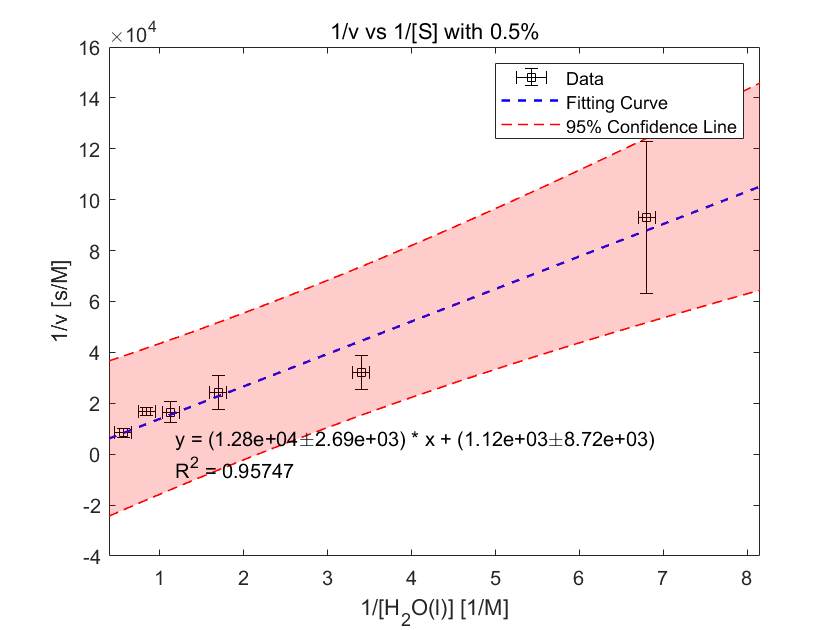
\includegraphics[width = 1.0\linewidth]{TOT_w_05.png}% Here is how to import EPS art
		\caption{\label{fig:TOT_w_05}0.5\% 데이터를 포함한 경우}
	\end{subfigure}
	\begin{subfigure}{0.4\textwidth}
		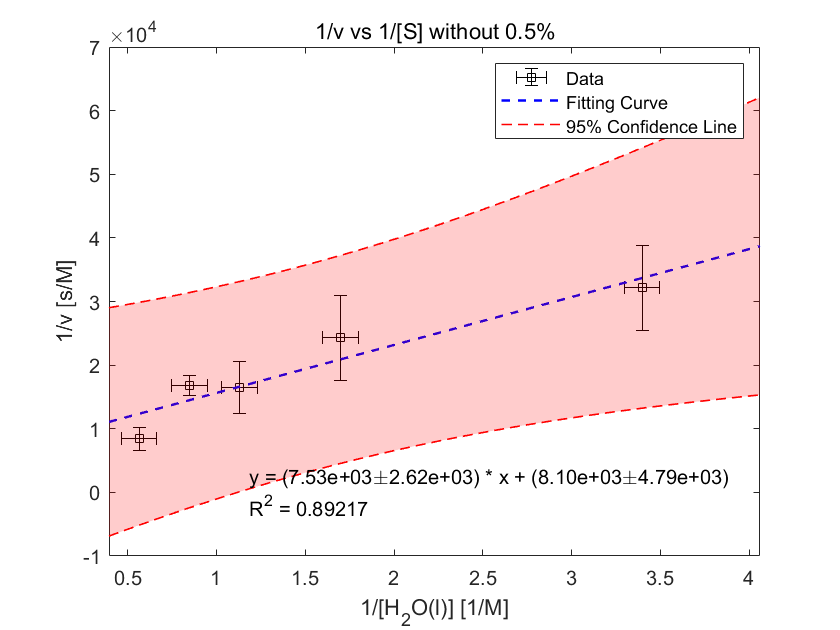
\includegraphics[width = 1.0\linewidth]{TOT_wo_05.png}% Here is how to import EPS art
		\caption{\label{fig:TOT_wo_05}0.5\% 데이터를 포함하지 않은 경우}
	\end{subfigure}
	\caption{\label{fig:TOT}Lineweaver-Burk equation에 fitting한 결과}
\end{figure*}

\begin{table}[]
\begin{tabular}{c|c|c|c} \hline \hline
& w/ 0.5\% Data & w/o 0.5\% Data  & 이론값[4] \\ \hline
$K_{m} [M]$ & $11\pm1$  & $0.92 \pm 0.01 $ & $1.1 \pm 0.25$ \\  \hline
오차& 900\% & 16\% & - \\  \hline \hline 
\end{tabular}
\caption{\label{tab:KM}Michaelis constant 측정 및 참값}
\end{table}

\begin{table}[]
\begin{tabular}{c|c|c} \hline \hline
& w/ 0.5\% Data & w/o 0.5\% Data\\ \hline
$V_{max} [mM/s]$ & $0.89 \pm 0.09 $  & $0.12 \pm 0.01 $\\  \hline \hline 
\end{tabular}
\caption{\label{tab:VMAX} $V_{max}$측정값}
\end{table}

\begin{figure}[htbp]
	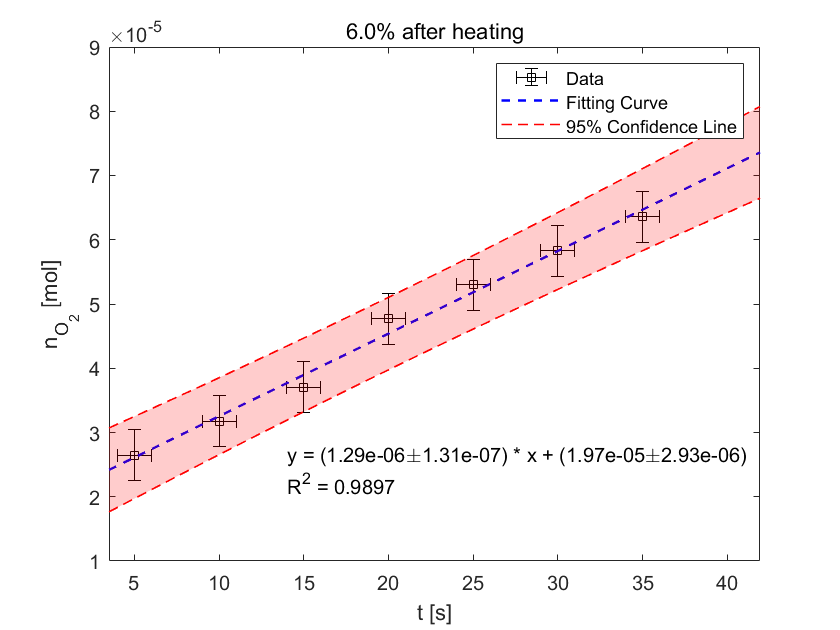
\includegraphics[width = 0.9\linewidth]{HEAT_60.png}% Here is how to import EPS art
	\caption{\label{fig:HEAT_60}6.0\% $\ch{H2O2}$ after heating}
\end{figure}

\section{\label{sec:level1}Conclusion \& Discussion}
속도측정값을 fitting했을 때 모두 높은 $R^{2}$값을 가져 실험의 재현도가 높음을 알 수 있다. 하지만  $0.5\%$농도에서의 데이터를 Lineweaver-Burk equation fitting에 포함시키는 경우 약 900\%의 큰 오차를 발생시킨다. 반면에 $0.5\%$농도에서의 데이터를 제외하는 경우 오차는 16\%로 크게 감소한다. 이것은 압력 측정 장비의 해상도가 약 $1.321hPa$인 반면 $0.5\%$농도에서 증가하는 압력의 기울기가 너무 작고 도중에 유출되는 산소기체가 많아 발생하는 현상으로 결론지었다. 따라서 산소 기체가 유출되기 전 빠르게 압력을 측정할 수 있는 고농도의 데이터만을 이용하고 해당 농도의 숫자를 늘려 $K_{m}$값을 계산하는 것이 정확한 결과를 도출할 수 있을 것으로 결론지었다. 

실험 측정값은 16\%오차내에서 높은 재현도와 정확도를 보여주었다. 또한 가열한 카탈레이스를 이용한 실험에서 시간당 발생하는 산소의 양이 감소하는 것을 확인하여 화학반응에서 촉매, 혹은 효소의 역할을 확인하였으며 가열시 발생하는 단백질의 변성에 의한 효소 기능 저하 또한 확인하였다. 하지만 실험도중 빠져나가는 산소기체로 인해 측정 실제 발생한 산소기체의 압력보다 더 낮은 값이 측정되어 큰 오차가 발생하였다. 이를 해결하기 위해 산적정을 수행하여 변화한 $\ch{H2O2}$의 양을 측정하여 더 정확한 반응속도를 측정할 수 있을 것이다. 이외에도 기체가 빠져나가는 현상을 방지하기 위해 수상치환하여 발생한 기체의 부피를 측정하는 방법 또한 있을 것이다.

\section{\label{sec:level1}Reference}
[1] 김. (2010, August 1). 캐털레이스의 반응속도. In \textit{일반화학실험} (1th ed., p. 186).

[2] Oxtoby, D., Gillis, H., \& Campion, A. (2007, April 2). Rates of Chemical and Physical Processes. In \textit{Principles of Modern Chemistry} (6th ed., pp .778-780). Cengage Learning.

[3] Garrett, R. H., \& Grisham, C. M. (2002, January 1). Enzyme Kinetics. In \textit{Principles of Biochemistry} (pp. 442-443). Cengage Learning.

[4]Jones, P., \& Suggett, A. (1968, December 1). The catalase–hydrogen peroxide system. A theoretical appraisal of the mechanism of catalase action. \textit{Biochemical Journal}, 110(4), 621–629. https://doi.org/10.1042/bj1100621

[5] Garrett, R. H., \& Grisham, C. M. (2002, January 1). Proteins: Their Biological Functions and Primary Structure. In \textit{Principles of Biochemistry} (pp. 115-119). Cengage Learning.

[6] Garrett, R. H., \& Grisham, C. M. (2002, January 1). Chemistry Is the Logic of Biological Phenomena. In \textit{Principles of Biochemistry} (p. 20). Cengage Learning.



\end{document}
%
% ****** End of file apssamp.tex ******
